\documentclass[a4paper,11pt]{article}
\usepackage{a4wide,amsmath,ngerman,url,graphicx}
\usepackage[utf8]{inputenc}
\parskip4pt
\parindent0pt

\newcommand{\br}[1]{\left(#1\right)}
\newcommand{\erf}{\mathrm{erf}}
\newcommand{\m}{\cdot}

\title{Analyse der Coronastatistiken. Teil 3} 
\author{Hans-Gert Gräbe, Leipzig}
\date{Version vom 27. Juni 2020}

\begin{document}
\maketitle

Corona ist vorangeschritten, die „Corona-Feuerwehr“ hat -- wenigstens in den
meisten mitteleuropäischen Ländern -- den „Flächenbrand“ in den Griff bekommen
und ist dazu übergegangen, einzelne Glutnester und neu auf"|flammende Hotspots
schnell und konsequent zu bekämpfen sowie die Außengrenzen scharf unter
Kontrolle zu halten.  Wir sind also zu einem anderen Krisenbekämpfungsmodus
übergegangen, was auch eine etwas andere Modellierung erfordert. Dazu aber
erst im nächsten Beitrag.

In diesem Beitrag wollen wir uns die mathematischen Hintergründe medialer
„Sternschnuppen“ etwas näher anschauen, die in der öffentlichen Debatte
kurzzeitig hell leuchteten und dann ebenso schnell wieder aus dem Verkehr
gezogen wurden, während die Daten der (privaten) JHU noch immer die Basis für
die täglichen Wasserstandsmeldungen zu positiv Getesteten $p(t)$ und
Verstorbenen $v(t)$ bilden, während die von der JHU ebenfalls übermittelte
Zahl der Genesenen $g(t)$ in der Zahl der aktuell Infizierten\footnote{Genauer
  sind es die Infizierten unter den Getesteten, die Genesenen unter den
  Getesteten usw. Allein bei den Verstorbenen kann man davon ausgehen, dass
  sie sämtlich irgendwann getestet wurden. Da sich alle weiteren Rechnungen
  auf die JHU-Zahlen als Referenz beziehen, ist stets „unter den Getesteten“
  hinzuzufügen, auch wenn dies nicht jedesmal ausdrücklich betont ist.}
$i(t)=p(t)-g(t)-v(t)$ enthalten ist, die aber in der Berichterstattung zu
Gunsten der über 7 Tage gemittelten Zahl der Neuinfektionen $\Delta
p(t)=p(t)-p(t-1)$ unerwähnt bleibt. Beide Zahlen hängen aber relativ eng
zusammen, da wir bei einer durchschnittlichen Genesungsdauer von
$T=16\,..\,21$ Tagen (siehe unten, die Werte streuen allerdings stark) davon
ausgehen können, dass in einer ersten Näherung $i(t)=p(t)-p(t-T)$ gilt.

Dieser Text ist eine Fortschreibung der ersten beiden Teile. Die dortigen
Beschreibungen der allgemeinen Rahmenbedingungen werden als bekannt
vorausgesetzt. Die wesentlichen Größen habe ich aber gerade noch einmal
rekapituliert. 

\section{Die „Verdoppelungsdebatte“}

Anfang April 2020 kommt eine Diskussion hoch, dass man die rigiden
Beschränkungen erst aufheben könne, wenn „die Verdopplungszeit der Infektionen
größer als 14 Tage“ sei.  Maß kann auch hier nur die Zahl der positiv
Getesteten sein. 

So meldet zum Beispiel der Deutschlandfunk am 04.04.2020\footnote{\raggedright
  \url{https://www.deutschlandfunk.de/covid19-verdopplungszeit-der-coronavirus-infektionen-in.1939.de.html?drn:news_id=1117169}}
\begin{quote}
  Die Verdopplungszeit der Ausbreitung von Coronavirus-Infektionen in
  Deutsch"|land hat sich in den vergangenen Tagen verlangsamt.

  Für ganz Deutschland liegt sie nun bei 11{,}2 Tagen. Die Lage in den
  Bundesländern ist unterschiedlich. In den großen Flächenländern liegt die
  Verdopplungszeit in Nordrhein-Westfalen bei 13{,}1 Tagen, in
  Baden-Württemberg bei 12{,}5 Tagen und in Bayern bei 9{,}7 Tagen. In Berlin
  sind es inzwischen 12{,}8 Tage, in Hamburg 12{,}4. Im Saarland hingegen
  liegt die Verdoppelungszeit bei 5{,}5 Tagen, in Sachsen bei 11{,}0 Tagen.
\end{quote}
Auch wenn dies nicht immer deutlich wird, bezieht sich die Verdopplungszeit
$v_t$ auf die kumulierten Daten $p(t)$ und steigt deshalb bereits durch die
schiere Masse der positiv Getesteten.  Ist $y(t)=mt+n$ ein linearer
Zusammenhang, so ergibt sich $v_t=\frac{y(t)}{m}$. Für einen annähernd
linearen Zusammenhang kann man also $v_t=\frac{y(t)}{y'(t)}$ als Schätzung
nehmen.  Die Zahl lässt sich auch aus unseren Daten leicht berechnen: Ist
$y_t=p(t)$ die kumulierte Zahl der positiv Getesteten am Tag $t$ und
$d_t=p(t)-p(t-1)$ die Zahl der (getesteten) Neuinfektionen, so ist nach
$v_t=\frac{y_t}{d_t}$ Tagen eine Verdopplung der positiv Getesteten erreicht,
die Zuwachsrate $d_t$ über diesen Zeitraum als konstant vorausgesetzt.  Beide
Datenreihen (Stand 10.04.2020) hatten wir schon in einem früheren Teil
extrahiert, so dass wir eine einfache Funktion \texttt{doublePlot(Land)}
schreiben können, um die folgenden Plots zu erzeugen. Auf der Abszisse ist der
Tag des Jahres 2020 aufgetragen, auf der Ordinate die berechnete
Verdopplungszeit. 
\begin{center}  
  \begin{minipage}{.33\textwidth}\centering
    \includegraphics[width=\textwidth]{Italy-DP.png}\\[1em] {Italien}
  \end{minipage}\hfill
  \begin{minipage}{.33\textwidth}\centering
    \includegraphics[width=\textwidth]{Germany-DP.png}\\[1em] {Deutschland}
  \end{minipage}\hfill
  \begin{minipage}{.33\textwidth}\centering
    \includegraphics[width=\textwidth]{Austria-DP.png}\\[1em] {Österreich}
  \end{minipage}
\end{center}

\section{Genesungsdauer}

Eine wichtige Größe für die Abschätzung der Infektionswirkung in Populationen
ist die Frage, wie lange ein einzelnes Individuum in der Lage ist, andere
anzustecken.  Wir bezeichnen diese durchschnittliche Zeit $T$ als
\emph{Genesungsdauer}. Diese Größe ist eine \emph{innere} Größe des
Infektionsgeschehens und deshalb weitgehend\footnote{Sozial ist der Zustand
  der Intensivmedizin, denn diese wendet den Tod einzelner Individuen ab, was
  $T$ leicht vergrößert. Das bleibt hier außer Betracht.} unabhängig von den
sozialen Randbedingungen.

Man kann sie deshalb aus den Daten verschiedener Länder einheitlich bestimmen,
wenn man die beiden Kurven $p(t)$ (positiv Getestete) und $g(t)+v(t)$
(Genesene und Verstorbene) hernimmt und schaut, wie groß der Abstand zwischen
beiden ist, etwa, indem der Tag bestimmt wird, wo jede der beiden Kurven einen
gewissen Schwellenwert überstiegen hat.

Hier das Ergebnis meiner Rechnungen auf den JHU-Daten für verschiedene
europäische Staaten und verschiedene Schwellwerte ($min$ bis $max$ in
Tausenderschritten bzw. für Österreich in Hunderterschritten -- es wurde ein
Teil der Kurven ausgesucht, in denen der Verlauf weitgehend linear war), $K$
eine Schätzung für den Sättigungswert der Kurve $p(t)$ (Stand 27.06.2020).

\begin{center}
  \begin{tabular}{|c|c|c|c|c|}\hline
    Land   & min..max & $K$ & Durchschnitt \\\hline
    Deutschland & $5\m10^4\dots 15\m10^4$ & $20\m 10^4$ & 15.5\\
    Italien & $5\m10^4\dots 15\m10^4$ & $25\m 10^4$ & 29.4\\
    Spanien & $5\m10^4\dots 15\m10^4$ & $25\m 10^4$ & 18.5\\
    Österreich & $5\m10^3\dots 12\m10^3$ & $2\m 10^4$ & 16.8\\\hline
  \end{tabular}
\end{center}

\section{$R_0$-Wert unter 1?}

Wikipedia erklärt die Größe wie folgt: „Die Basisreproduktionszahl $R_0$
... und die Nettoreproduktionszahl $R$ sind Begriffe aus der
Infektionsepidemiologie.  $R_0$ gibt an, wie viele Menschen von einer
infektiösen Person durchschnittlich angesteckt werden, wenn kein Mitglied der
Population gegenüber dem Erreger immun ist“. Weiter wird betont, dass „$R_0$
keine biologische Konstante für einen Erreger ist, da sie wesentlich auch von
anderen Faktoren wie den Umweltbedingungen und dem Verhalten der infizierten
Bevölkerung beeinflusst wird“.  Dort sind auch eine Reihe mathematischer
Modelle aufgeführt, aus denen sich $R_0$ schätzen lässt.

Ist $r$ die Rate, mit der ein Infizierter durchschnittlich andere Personen
\emph{pro Tag} ansteckt, so ergibt sich $R_0=r\m T$, wobei $T$ für die
durchschnittliche Zeit steht, in der eine Person infektiös ist. Wir  hatten
diese Größe im letzten Abschnitt mit etwa $T=18$ geschätzt. $r$ selbst ergibt
sich aus den JHU-Zahlen und dem Zusammenhang $\Delta\,p(t)=r\m i(t)$ zwischen
Neuinfektionen und der aktuellen Zahl der Infizierten.  

Berechnet man aus den beiden Datenreihen den Quotienten $\Delta\,p(t)/i(t)$
und multipliziert diesen mit $T=18$, so ergibt sich für verschiedene Länder
ein spannendes Bild, das in Teilen wenig mit den Erwartungen zu tun hat, und
damit möglicherweise auch mehr über die Informationspolitik als die wirklichen
Verhältnisse aussagt.  Die blauen Punkte sind die Rohdaten, die grüne Linie
jeweils der über 7 Tage geglättete Durchschnittsverlauf. Dargestellt ist der
Verlauf ab Tag 100, also dem 9.4.2020.

\begin{center}
  \begin{minipage}{.3\textwidth}\centering
    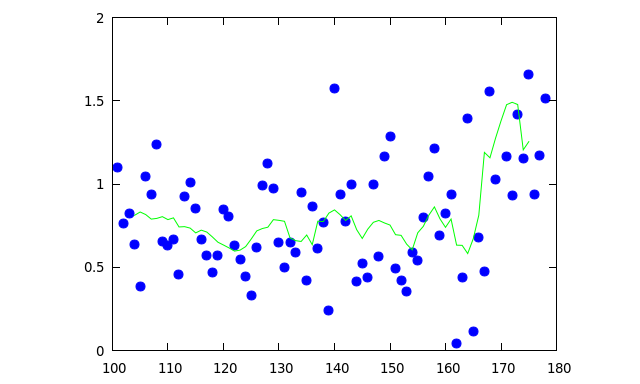
\includegraphics[width=\textwidth]{Germany-R.png}\\[1em] {Deutschland}
  \end{minipage}\hfill
  \begin{minipage}{.3\textwidth}\centering
    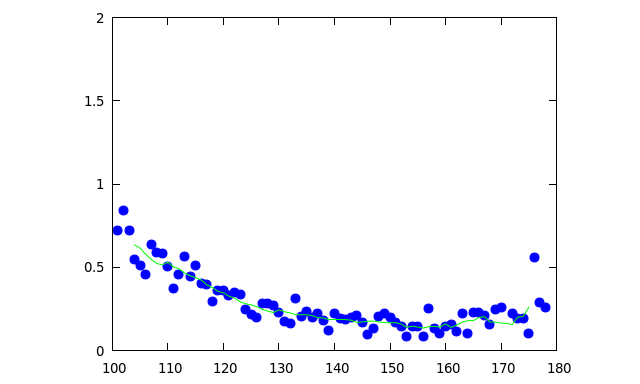
\includegraphics[width=\textwidth]{Italy-R.png}\\[1em] {Italien}
  \end{minipage}\hfill
  \begin{minipage}{.3\textwidth}\centering
    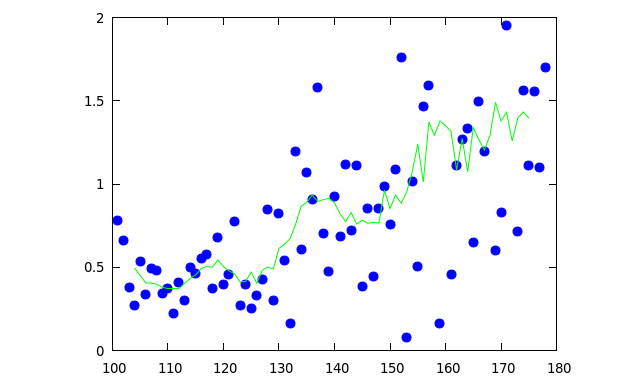
\includegraphics[width=\textwidth]{Austria-R.png}\\[1em] {Österreich}
  \end{minipage}

  \begin{minipage}{.3\textwidth}\centering
    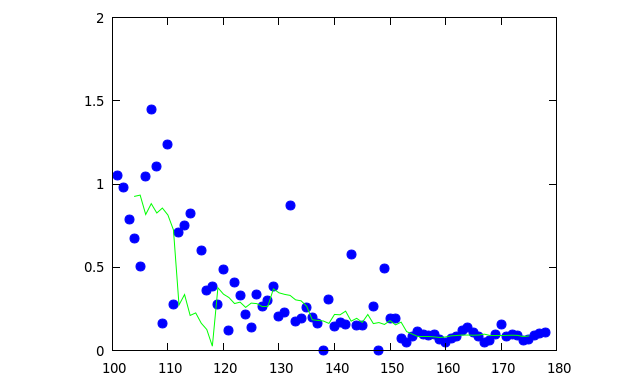
\includegraphics[width=\textwidth]{Spain-R.png}\\[1em] {Spanien}
  \end{minipage}\hfill
  \begin{minipage}{.3\textwidth}\centering
    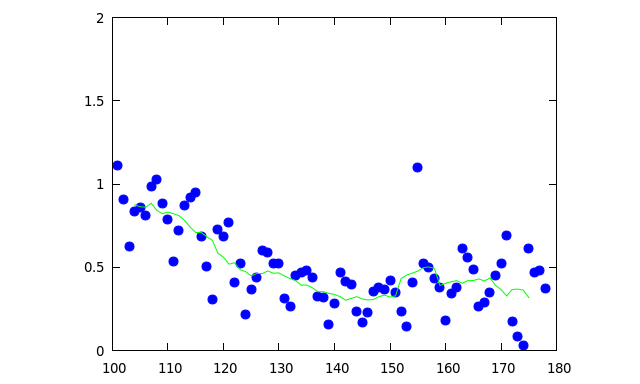
\includegraphics[width=\textwidth]{Sweden-R.png}\\[1em] {Schweden}
  \end{minipage}\hfill
  \begin{minipage}{.3\textwidth}\centering
    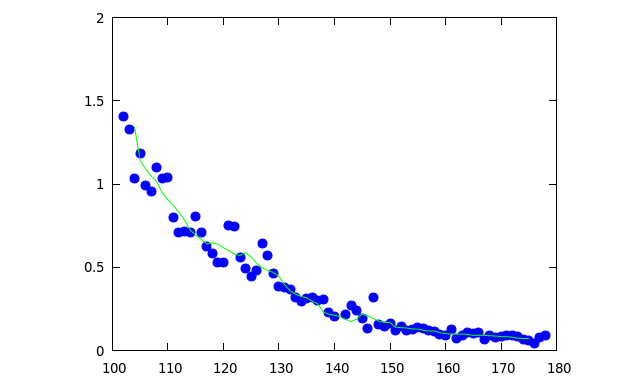
\includegraphics[width=\textwidth]{UK-R.png}\\[1em] {Großbritannien}
  \end{minipage}
\end{center}

\end{document}
